\chapter{Teoria semiclassica dell'interazione radiazione-materia}
\graphicspath{{./cap_2/images/}}

\section{Transizioni elettroniche indotte da perturbazioni dipendenti dal tempo}
Consideriamo l'atomo idrogenoide e indichiamo con $\psi(\*r,t)$ la funzione d'onda dell'elettrone più esterno (elettrone ottico) che compie transizioni. Trascuriamo lo spin dell'elettrone.\\
In assenza di perturbazioni $\psi$ evolve secondo l'equazione:
\begin{equation*}
    i\hbar \frac{\p \psi}{\p t} = \widehat{H}_0 \psi \quad \text{con} \quad \widehat{H}_0 \equiv -\frac{\hbar^2}{2m} \N^2 + V(\*r)
\end{equation*}

Indichiamo con $\lve{n} \equiv u_n(\*r)$ ed $E_n$ le autofunzioni normalizzabili (stati legati dell'atomo) e le energie (autovalori) di $\widehat{H}_0$:
\begin{equation}\label{eq: eq auto non perturbata}
    \widehat{H}_0 \lve{n} = E_n \lve{n}
\end{equation}

Ricordiamo che:
\begin{equation*}
    \langle n | m \rangle \equiv \intinf u_n^*(\*r) \; u_m(\*r) \; d\*r = \delta_{n,m} = \begin{cases}
        1\quad n = m\\
        0 \quad n \neq m
    \end{cases}
\end{equation*}

Supponiamo che l'elettrone interagisca con una perturbazione esterna (ad esempio, l'atomo è investito da un'onda e.m.). La perturbazione è descritta da un operatore auto-aggiunto $\hat{H_p}$ che assumiamo della forma:
\begin{equation}\label{eq: ham perturbata}
    \widehat{H}_p = f(t) \widehat{p}
\end{equation}

dove $f(t)$ è in funzione quasi monocromatica nel tempo della forma seguente:
\begin{equation*}
    f(t) = \frac{1}{2} \left[ A(t) e^{i\w t} + c.c. \right]
\end{equation*}
con $A(t)$ lentamente variabile di periodo $T =  \frac{2\pi}{\omega}$.

$\widehat{p}$ è un operatore indipendente dal tempo che quindi agisce sulle sole coordinate spaziali $\*r$.\\
In presenza della perturbazione l'equazione di Schr\"{o}dinger diventa:
\begin{equation} \label{eq: schrod perturbata}
    i\hbar \frac{\p \psi}{\p t} = \left(\widehat{H}_0 + \widehat{H}_p\right)\psi
\end{equation}

essendo $\widehat{H} = \widehat{H}_0 + \widehat{H}_p$ l'hamiltoniana complessiva.\\
Se si trascurano i processi di ionizzazione, ad ogni istante $t$, $\psi(\*r,t)$ può essere sviluppata in serie degli autostati \lv{n} di $\widehat{H}_0$ cioè:
\begin{equation}\label{eq: fun donda}
    \psi(\*r,t) = \sum_n C_n(t) e^{-i\frac{E_n}{\hbar}t} \lve{n}
\end{equation}

Sostituendo l'\textit{Ansatz} (assunzione) \eqref{eq: fun donda} nella \eqref{eq: schrod perturbata} si ha:
\begin{equation*}
    i\hbar \sum_n \left[\frac{d C_n}{d t} - i\frac{E_n}{\hbar} C_n \right] e^{-i\frac{E_n}{\hbar}t} \lve{n} = \sum_n C_n [\widehat{H}_0 + \widehat{H}_p] e^{-i\frac{E_n}{\hbar}t} \lve{n}
\end{equation*}

\begin{equation*}
    i\hbar \sum_n \dot{C}_n e^{-i\frac{E_n}{\hbar}t} \lve{n} + \cancel{i\hbar \sum_n C_n e^{-i\frac{E_n}{\hbar}t} \left(-i\frac{E_n}{\hbar}\right) \lve{n}} = \cancel{\sum_n C_n e^{-i\frac{E_n}{\hbar}t} \widehat{H}_0 \lve{n}} + \sum_n C_n e^{-i\frac{E_n}{\hbar}t} \widehat{H}_p \lve{n}
\end{equation*}

sostituendo \eqref{eq: eq auto non perturbata}, \eqref{eq: ham perturbata} e semplificando si ottiene:
\begin{equation*}
    i\hbar \sum_n \dot{C}_n e^{-i\frac{E_n}{\hbar}t} \lve{n} = \sum_n C_n e^{-i\frac{E_n}{\hbar}t} f(t) \widehat{p} \lve{n}
\end{equation*}

Moltiplicando per $\langle m|$ e tenendo conto che $\langle m|n\rangle = \delta_{n,m}$ si ha:
\begin{equation*}
    i\hbar \dot{C}_m e^{-i\frac{E_m}{\hbar}t} = f(t) \sum_n \langle m|\widehat{p}|n\rangle C_n e^{-i\frac{E_n}{\hbar}t}
\end{equation*}

ovvero:
\begin{equation*}
    i\hbar \dot{C}_m = f(t) \sum_n p_{m,n} C_n e^{-i\frac{(E_n - E_m)}{\hbar}t}
\end{equation*}

avendo posto:
\begin{equation*}
    p_{m,n} \equiv \langle m|\widehat{p}|n\rangle \equiv \intinf u_m^*(\*r) \; \widehat{p} \; u_n(\*r) \; d\*r
\end{equation*}
definito elemento di matrice di perturbazione.\\

Si noti che $p_{n,m}$ è una matrice hermitiana, ovvero $p_{n,m} = p_{n,m}^*$.\\
\\
\textit{Qual è il significato fisico di $C_n(t)$?}
\begin{indentedpar}{1cm}
$|C_n(t)|^2$ è la probabilità che al tempo $t$ l'elettrone si trovi sullo stato \lv{n} con energia $E_n$.
\end{indentedpar}
\noindent
\textit{Qual è l'effetto della perturbazione?}
\begin{indentedpar}{1cm}
Se non ci fosse la perturbazione, cioè se $f(t) = 0$ allora $|C_n(t)|^2 = cost$.
Quindi, se al tempo $t=0$ l'elettrone, con certezza, si trova su un dato livello $\bar{n}$ cioè $C_n(0) = \delta_{n,\bar{n}}$ allora l'elettrone rimane sul livello \lv{\bar{n}} (stato stazionario).

In presenza di una perturbazione i $C_n(t)$ variano nel tempo. La perturbazione induce cioè transizioni tra i diversi stati stazionari dell'atomo.
\end{indentedpar}

Fissando l'attenzione al caso dell'atomo a due livelli \lv{1} e \lv{2}, chiamando $\omega_0 = \frac{E_2 - E_1}{\hbar}$ la frequenza di risonanza della transizione $\lve{1} \leftrightarrow \lve{2}$ e notando che gli elementi diagonali della matrice di perturbazione $p_{1,1}$ e $p_{2,2}$ sono nulli si ha:
\begin{empheq}[box=\eqbox]{equation*}
    \begin{cases}
        i\hbar \dot{C_1} = f(t) \; p_{12} \; C_2 \; e^{-i\omega_0 t} \qquad \textbf{equazione del sistema}\\
        i\hbar \dot{C_2} = f(t) \; p_{21} \; C_1 \; e^{i\omega_0 t} \qquad \textbf{ di un atomo a due livelli}
    \end{cases}
\end{empheq}

Specifichiamo le condizioni iniziali per una perturbazione piccola.\\
Si supponga che al tempo $t=0$ l'elettrone sia con certezza sul livello \lv{2} e che  quindi $C_1(0) = 0$ e $C_2(0) = 1$ e, inoltre, si supponga che la perturbazione sia quasi monocromatica con frequenza $\w\simeq\omega_0$ ovvero $f(t) = \frac{1}{2} \left( A(t) e^{-i\omega t} + \,c.c.\right)$ con $A(t)$ lentamente variabile su un intervallo $\frac{2\pi}{\omega}$.

Se la perturbazione è debole (ovvero se $A \rightarrow 0$) e se il tempo di interazione ($0,t$) non risulta troppo grande allora $C_1(t)$ e $C_2(t)$ non varieranno troppo rispetto ai valori imperturbati, ovvero:
\begin{equation*}
    |C_1(t)|^2 << 1 \qquad |C_2(t)|^2 \simeq 1
\end{equation*}

Possiamo in tale ipotesi trascurare la seconda equazione nel sistema e risolvere la prima:
\begin{equation*}
    i\hbar \dot{C_1} = p_{1,2} \; f(t) \; C_2 \; e^{-i\omega_0 t} \approx p_{1,2} \; f(t) \; e^{-i\omega_0 t}
\end{equation*}

deducendo che l'evolvere di $C_1$ non dipende da $C_2$.
Risolvendo per $C_1(t)$ si ottiene:
\begin{equation*}
    C_1(t) = \frac{p_{1,2}}{i\hbar} \int_0^t f(t') \; e^{-i\omega_0 t'} dt'
\end{equation*}

Se spengo la perturbazione al tempo $t = T$ la probabilità di trovare l'elettrone sul livello \lv{1} vale:
\begin{equation}\label{eq: probab c1}
    |C_1(t)|^2 = \frac{|p_{1,2}|^2}{\hbar^2} \left|\int_0^T f(t') \; e^{-i\omega_0 t'} dt'\right|^2
\end{equation}

È quindi possibile introdurre una\textbf{ probabilità di transizione} $W_{21}$ da $\lve{2} \rightarrow \lve{1}$ nell'unità di tempo così definita:
\begin{equation*}
    W_{21} = \lim_{T \rightarrow \infty} \frac{|C_1(T)|^2}{T}
\end{equation*}

Sostituendo $f(t) = \frac{1}{2} \left[ A(t) e^{-i\omega t} + c.c.\right]$ nell'integrale della \eqref{eq: probab c1} si ha:
\begin{equation*}
    \left|\int_0^T f(t') e^{-i\omega_0 t'} dt'\right|^2 = \left|\underbrace{\frac{1}{2} \int_0^T A(t') e^{i(\omega - \omega_0) t'} dt'}_\text{termine risonante} + \underbrace{\frac{1}{2} \int_0^T A^*(t') e^{-i(\omega + \omega_0) t'} dt'}_\text{termine anti-risonante} \right|^2
\end{equation*}

\textbf{Nota.}\\
Se $A(t) = 1$ e $\omega = \omega_0$ si hanno:
\begin{equation*}
    \int_0^T  dt' = T \quad \text{termine risonante}
\end{equation*}
\begin{equation*}
    \int_0^T e^{-2i\omega_0 t'} dt' = \frac{1 - e^{-2i\omega_0 T}}{2i \omega_0} \quad \text{termine anti-risonante}
\end{equation*}

Trascurare il termine anti-risonante è detta \textbf{approssimazione di onda rotante}.
Facendo questa approssimazione quindi si ottiene:
\begin{empheq}[box=\eqbox]{equation}\label{eq: regola di fermi}
    W_{21} = \frac{|p_{1,2}|^2}{4\hbar^2} S(\omega - \omega_0) \quad \text{regola d'oro di Fermi}
\end{empheq}

avendo posto:
\begin{empheq}[box=\eqbox]{equation*}
    S(\D \w) \equiv \lim_{T \rightarrow \infty} \frac{1}{T} \left| \int_0^T A(t') e^{i(\D\w) t'} dt' \right|^2 \quad \text{spettro di potenza dell'inviluppo A(t)}
\end{empheq}

\textbf{Osservazioni.}
\begin{enumerate}
    \item Se $C_1(0) = 1$ e $C_2(0) = 0$ applicando la matrice di perturbazione si ha che:
    \begin{equation*}
        W_{12} = \lim_{T \rightarrow \infty} \frac{|C_2(T)|^2}{T} = W_{21}
    \end{equation*}

    \item Un altro metodo per scrivere la Regola d'oro di Fermi è attraverso le funzioni di autocorrelazione:
    \begin{equation*}
        A_T(t) = \begin{cases}
            A(t) \quad 0 < t < T\\
            0 \quad \text{altrimenti} 
        \end{cases}    
    \end{equation*}
    e la funzione di autocorrelazione:
    \begin{equation*}
        R(t) \equiv \intinf A_T(t) A_T^*(t - \tau) dt
    \end{equation*}
    allora è facile vedere che:
    \begin{equation*}
        S(\D\w) = \intinf R(\tau) e^{i\D\w\tau} d\tau
    \end{equation*}
    ovvero lo spettro di potenza $S(\D\w)$ di $A(t)$ è l'integrale di Fourier della sua funzione di autocorrelazione.
    
    \item La teoria di perturbazione è valida quando è verificata la seguente condizione:
    \begin{equation*}
        W_{21}T << 1
    \end{equation*}
    infatti:
    \begin{equation*}
        W_{21} = \frac{|C_1(T)|^2}{T} \Longrightarrow |C_1(T)|^2 = W_{21}T << 1
    \end{equation*}
\end{enumerate}

\begin{example}
Perturbazione rigorosamente monocromatica.\\
Supponiamo $f(t) = \cos(\omega t)$ cioè $A(t) = 1$. In tal caso lo spettro di potenza $S$ vale:
\begin{align*}
    S(\D \w) &= \lim_{T \rightarrow \infty} \frac{1}{T} \left| \int_0^T e^{i(\D\w) t} dt \right|^2\\
    &= \lim_{T \rightarrow \infty} \frac{1}{T} \left|\frac{e^{i\D\omega T} - 1}{i\D w} \right|^2\\
    &= \lim_{T \rightarrow \infty} \frac{1}{T} \left|\frac{e^{\frac{i\D\omega T}{2}} \left(e^{\frac{i\D\omega T}{2}} - e^{\frac{-i\D\omega T}{2}} \right)}{i\D w} \right|^2\\
    &= \lim_{T \rightarrow \infty} \frac{1}{T} \left|\frac{4 \sin^2\left(\frac{\D\omega T}{2}\right)}{\D w^2} \right|^2\\
    &= \lim_{T \rightarrow \infty} T \left|\frac{\sin^2\left(\frac{\D\omega T}{2}\right)}{\left(\frac{\D w T}{2}\right)^2} \right|^2
\end{align*}

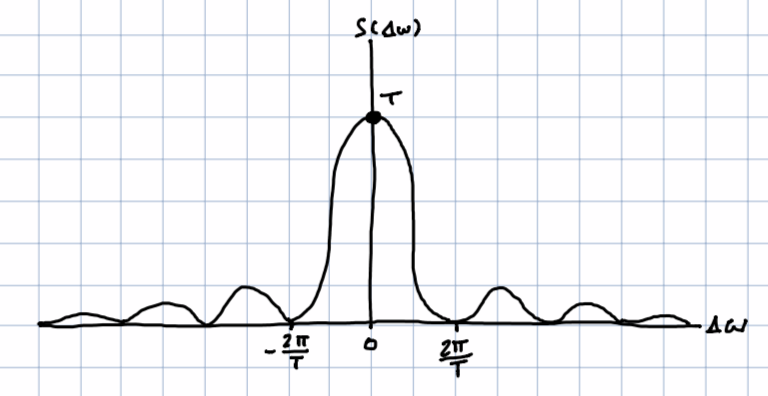
\includegraphics[width=5cm, center]{sinc}

Studiamo la funzione $G(\D \w) = T sinc^2\left(\frac{\D \omega T}{2}\right)$ al crescere di T.

Si noti che l'area:
\begin{equation*}
    \intinf G(\D \w) = T \intinf sinc^2\left(\frac{\D \omega T}{2}\right) = T \frac{2}{T} \intinf \frac{sin^2\xi}{\xi^2} d\xi = 2\pi
\end{equation*}

Nel limite $T \rightarrow \infty$:
\begin{equation*}
    G(\D \w) = \begin{cases}
        \infty \quad \D\omega = 0\\
        0 \quad \D\omega \neq 0
    \end{cases}
\end{equation*}
cioè lo spettro di potenza tenderà ad una delta di Dirac di area $2\pi$ per $\Delta \omega \rightarrow 0$.

In definitiva $\Delta S(\Delta \w) = 2\pi \delta(\Delta \w)$:
\begin{equation*}
    W_{12} = W_{21} = \pi \frac{|p_{1,2}|^2}{2\hbar^2} \delta(\omega - \omega_0) \quad \text{per perturbazione monocromatica}
\end{equation*}
\end{example}

\begin{example}Onda quasi monocromatica con salti di fase casuali\\
Supponiamo che $f(t) = \cos(\omega t +\varphi(t))$ con $\varphi(t)$ costante a tratti con discontinuità a valori casuali distribuiti fra $(0,2\pi)$, ad intervalli $\tau$ con $\tau$ variabile aleatoria. 
\begin{wrapfigure}{R}{0.3\textwidth}
    \centering
    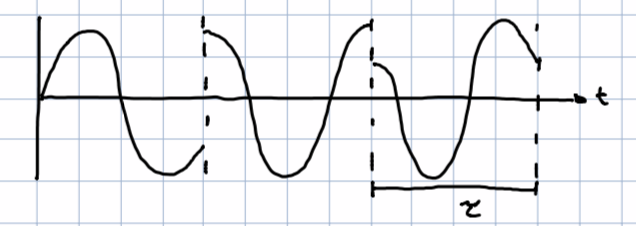
\includegraphics[width=0.9\linewidth]{phase_jumps}
\end{wrapfigure}
Supponiamo inoltre che $\varphi$ abbia distribuzione di probabilità esponenziale:
\begin{equation*}
    \varphi(\tau) = \frac{1}{\tau_c} e^{-\frac{\tau}{\tau_c}}
\end{equation*}
dove $\tau_c$ è il valore medio.

Calcoliamo lo spettro di potenza $S(\D \w)$ come integrale di Fourier della funzione di autocorrelazione $R(\tau)$\footnote{Per il calcolo di $R(\tau)$ vedi \textit{Principles of lasers} Appendice del capitolo 12}.

Il risultato è:
\begin{equation*}
R(\tau) = e^{-\frac{|\tau|}{\tau_c}}
\end{equation*}
%grafico
Calcolo lo spettro di potenza:
\begin{align*}
    S(\D \w) &= \intinf e^{-\frac{|\tau|}{\tau_c}} e^{i\D\w\tau} d\tau\\
    &= \int_0^{+\infty} e^{-\frac{|\tau|}{\tau_c}} e^{i\D\w\tau} d\tau + \int_{-\infty}^0 e^{\frac{|\tau|}{\tau_c}} e^{i\D\w\tau} d\tau\\
    &= \frac{e^{\left(i\D\omega - \frac{1}{\tau_c}\right)\tau|_0^{+\infty}}}{i\D\omega - \frac{1}{\tau_c}} + \frac{e^{\left(i\D\omega + \frac{1}{\tau_c}\right)\tau|_{-\infty}^0}}{i\D\omega + \frac{1}{\tau_c}}\\
    &= -\frac{1}{i\D\omega - \frac{1}{\tau_c}} + \frac{1}{i\D\omega + \frac{1}{\tau_c}}\\
    &= \frac{\tau_c}{1 - i\D\w\tau_c} + \frac{\tau_c}{1 + i\D\w\tau_c}\\
    &= \frac{2\tau_c}{1 + (\D\w\tau_c)^2}
\end{align*}

che possiamo riscrivere:
\begin{equation*}
    S(\D\w) = 2\pi g_L(\D\w)
\end{equation*}

dove:
\begin{empheq}[box=\eqbox]{equation*}
    g_L\left(\D\w\right) = \frac{\tau_c}{\pi} \frac{1}{1 + (\D\omega \tau_c)^2} \quad \text{funzione lorentziana}
\end{empheq}

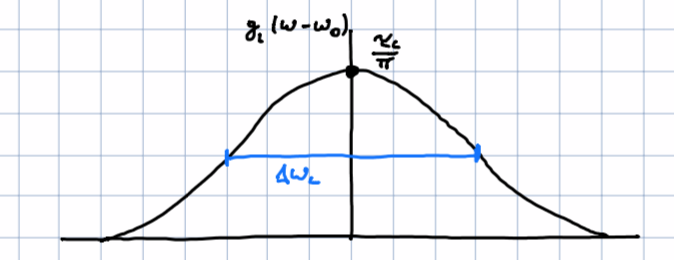
\includegraphics[width=5cm, center]{lorentziana}

È quindi facile vedere che $g_L$ è normalizzata: $\intinf g_L(\D\w) d\D\omega = 1$.

La lunghezza a metà altezza $FWHM$ della lorentziana vale:
\begin{equation*}
    g_L\left(\frac{\D\omega_L}{2}\right) = \frac{\tau_c}{2\pi}
\end{equation*}
ovvero vale
\begin{equation*}
    \D \omega_L = \frac{2}{\tau_c}
\end{equation*}
Pertanto per la regola d'oro di Fermi \eqref{eq: regola di fermi}
\begin{equation*}
    W_{12} = W_{21} = \frac{|p_{1,2}|^2}{4\hbar^2} S(\omega - \omega_0)
\end{equation*}

Il caso di onda perfettamente monocromatica è per la lorentziana il limite $\tau_c \rightarrow \infty$.\\
Ritroviamo il risultato dell'esempio.

L'espressione $W_{12} = W_{21}$ dalla teoria perturbativa è ben posta anche a risonanza ($\omega = \omega_0$) in quanto la lorentziana non ha la singolarità del seno cardinale.
\end{example}

\section{Assorbimento ed emissione stimolata: Calcolo di $W_{12} = W_{21}$}
Considero un atomo a due livelli investito da un'onda piana (quasi) monocromatica di frequenza $\w$, che si propaga nella direzione $z$ dello spazio con campo $\*E$ linearmente polarizzato in direzione $x$.

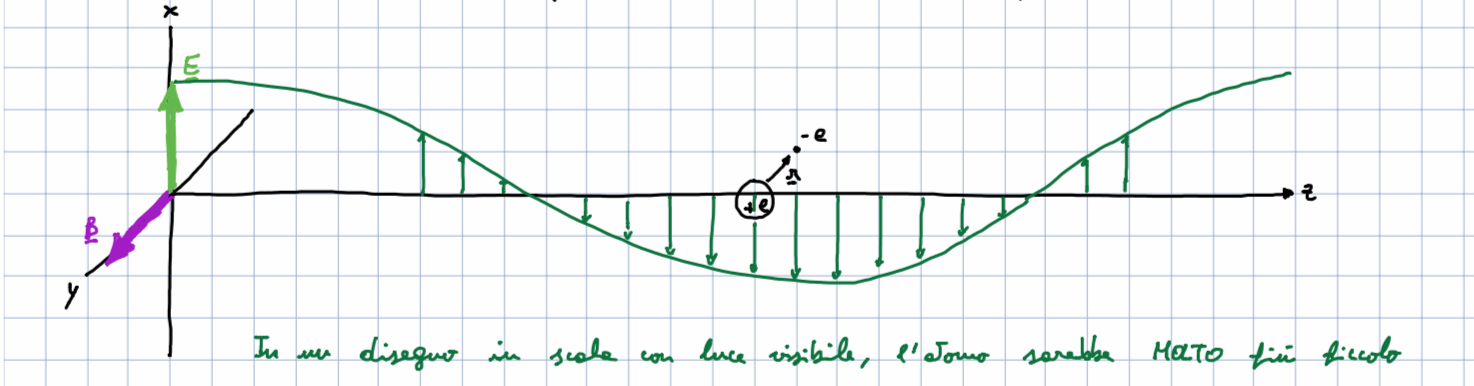
\includegraphics[width=12cm, center]{onda_mono_lin_pol}

L'elettrone dell'atomo risente, oltre che del potenziale nucleare, anche della forza di Lorentz:
\begin{equation*}
    \*F = -e\*E - e\*v\times\*B = -e\*E_x(z, t)\*u_x -e\*v\times \*u_y\*B_y(z, t)
\end{equation*}
L'hamiltoniana classica per un elettrone in un campo elettromagnetico è la seguente:
\begin{equation*}
    \widehat{H} = \frac{1}{2m} \left(\*p + q\*A\right)^2 + qV \qquad \N\cdot\*B = \N\cdot\N\times\*A = 0
\end{equation*}

Nell'approssimazione di dipolo elettrico assumiamo le seguenti ipotesi:
\begin{enumerate}
    \item Poiché l'elettrone è localizzato attorno al nucleo per una dimensione dell'ordine del raggio di Bohr $a_0 \propto 0.053 nm$ e la lunghezza d'onda nel visibile (rosso) è circa $\l \simeq 500 nm$ allora possiamo considerare il campo elettrico e il campo magnetico pressoché costanti. Posso quindi assumere, nell'espressione di $\*F$, $z=z_N$. Ovvero la coordinata $z$ è costante e pari alla posizione del nucleo.
    
    \item Per basse velocità $|\*v| << c$ è possibile trascurare la forza di Lorentz.
\end{enumerate}

Per queste ipotesi si ha che la forza che l'elettrone sente per effetto dell'onda e.m. è pari a:
\begin{equation}
    \*F(t) \simeq -e\*E_x(z_N, t)\*u_x
\end{equation}
la quale deriva dall'energia potenziale $H_p(x, t) = e x E_x(t)$.

Si noti che l'energia classica di dipolo elettrico in campo esterno è la seguente:
\begin{equation}
    H_p -\*{\mu} \cdot \*E
\end{equation}
dove $\*\mu = -e\*r$ è il momento di dipolo elettrico dell'atomo.

L'operatore quantistico di perturbazione è pertanto:
\begin{equation}
    \hat{H}_p = e x E_x(t) = f(t) \hat{p}
\end{equation}
dove $f(t) = E_x(t)$ e $\hat{p} \equiv e x = -\*\mu \cdot \*u_x$.

L'elemento di matrice di perturbazione che entra nella formula di $W_{12} = W_{21}$
\begin{equation}
    |p_{12}|^2 = |<1|e x|2>|^2 = \left|\intinf u_1^*(\*r) \; e x \; u_1(\*r) d\*r \right|^2
\end{equation}
ovvero $|p_{12}|^2 = |\mu_{12x}|^2$
dove si è definito l'elemento di matrice di dipolo elettrico della transizione $\lve{1} \rightarrow \lve{2}$:
\begin{equation}
    \*\mu_{12} \equiv <1|e\*r|2>
\end{equation}

Quindi, ad esempio, per onda rigorosamente monocromatica, cioè se $E_x(t) = E_x \cos(\w t)$:
\begin{equation}
    W_{12} = W_{21} = \frac{\pi |\mu_{12x}|^2 E_0^2}{2 \hbar^2} \delta(\w - \w_0)
\end{equation}

Se invece $E_x(t) = E_0 \cos(\w t + \varphi(t))$ similmente si ha:
\begin{equation}
    W_{12} = W_{21} = \frac{\pi |\*\mu_{12x}|^2 E_0^2}{2 \hbar^2} g_L(\w - \w_0)
\end{equation}
Nel caso si abbiano più atomi, il valore medio vale:
\begin{equation}
    \bar{W}_{12} = \bar{W}_{21} = \frac{\pi <|\*\mu_{12x}|^2> E_0^2}{2 \hbar^2} g_L(\omega - \omega_0)
\end{equation}
dove $<|\*\mu_{12x}|^2>$ è il valore medio $\frac{|\*\mu_{12x}^{(1)}|^2 + |\*\mu_{12x}^{(2)}|^2 + ... + |\*\mu_{12x}^{(n)}|^2}{N}$.

Se la distribuzione degli atomi nello spazio è isotropa:
\begin{equation}
    <|\*\mu_{12x}|^2> = <|\*\mu_{12y}|^2> = <|\*\mu_{12z}|^2>
\end{equation}

Del resto $|\*\mu_{12x}|^2 + |\*\mu_{12y}|^2 + |\*\mu_{12z}|^2 = |\*\mu_{12}|^2$ quindi mediando:
\begin{equation}
    <|\*\mu_{12x}|^2> + <|\*\mu_{12y}|^2> + <|\*\mu_{12z}|^2> = |\*\mu_{12}|^2
\end{equation}
e quindi:
\begin{equation}
    <|\mu_{12x}|^2> = \frac{|\mu_{12}|^2}{3}
\end{equation}

In definitiva:
\begin{empheq}[box=\eqbox]{equation*}
    W_{12} = W_{21} = \frac{\pi |\*\mu_{12}|^2 E_0^2}{6 \hbar^2} g_L(\w - \w_0)
\end{empheq}
Per tenere conto di tanti atomi è sufficiente dividere per 3 il modulo di $\*\mu_{12}$.

Con questa teoria si può studiare l'effetto sull'atomo della perturbazione dell'onda ma non è possibile sapere cosa succede all'onda (fotone creato, distrutto); per tenere conto di ciò è necessaria la teoria di seconda quantizzazione.

\textbf{Osservazioni.}\\
\begin{enumerate}
    \item Regole di selezione di dipolo elettrico:
    $W_{12} = W_{21}$ si annulla se l'elemento di matrice di transizione $ = 0$. In tal caso la transizione si dice proibita per dipolo elettrico, altrimenti è permessa.
    Negli atomi idrogenoidi $\hat{H}_0(-\*r) = \hat{H}_0(\*r)$ cioè è simmetrica per invarianza, per cui le autofunzioni $u_n(\*r) \equiv \lve{n}$ sono a parità definita, cioè:
    \begin{equation}
        u_n(-\*r) = u_n(\*r) \quad pari \qquad u_n(-\*r) = - u_n(\*r) \quad dispari
    \end{equation}
    Per cui:
    \begin{equation}
        \*\mu_{12} = \intinf u_1^*(\*r) \; e \*r \; u_1(\*r) dx dy dz = \begin{cases}
        0 \quad \text{se \lv{1} e \lv{2} stessa parità}\\
        \neq 0 \quad \text{se \lv{1} e \lv{2} parità opposta}
        \end{cases}
    \end{equation}
    Ci può essere transizione solo per autofunzioni di parità opposta. Questa proprietà dà origine alle cosiddette \textit{Regole di Selezione}, che per atomi idrogenoidi sono:
    \begin{equation}
        \Delta l = \pm 1 \quad \Delta j = 0, \pm 1 \quad \Delta m_j = 0, \pm 1
    \end{equation}
    Ad esempio transizioni tra stati \textit{s} e \textit{p} sono permesse per dipolo elettrico (non c'è nessun vincolo su \textit{n}).
    Queste regole sono valide nelle ipotesi dell'approssimazione di dipolo elettrico.
    
    \item Transizioni indotte per dipolo magnetico\\
    Se $\*\mu_{12} = 0$, i processi di assorbimento / emissione stimolata possono avvenire per interazioni di ordine superiore
    Mi limito a studiare il dipolo magnetico, l'energia classica di interazione è:
    \begin{equation}
        H_p = - \*\mu_m \cdot \*B
    \end{equation}
    dove $\*\mu_m = IS \*n = -\frac{e S}{T} \*n$ è il momento di dipolo magnetico calssico dell'elettrone orbitale e $\*B$ è il campo magnetico dell'onda, dove $S$ è l'area dell'orbita e T il periodo di rivoluzione.
    Detta $\alpha$ la velocità angolare:
    \begin{equation}
        \alpha = \frac{1}{2} r^2 \frac{d\theta}{dt} = \frac{1}{2} r^2 \dot{\theta} = costante
    \end{equation}
    Quindi $S = \int_0^T \alpha dt = \alpha T$ per cui $\*\mu = -e \alpha \*n$.
    Il momento angolare dell'elettrone è $\*L = \*r \times m\*v = mr^2 \dot{\theta} \*n = 2m \alpha \*n$ quindi:
    \begin{equation}
        \*\mu_{m} = -\frac{e}{2m} \*L
    \end{equation}
    L'energia classica di interazione è quindi ($\*B = B_y \*\mu_y = B_0 cos(\w t + \varphi(t))$):
    \begin{equation}
        H_p = -\*mu \cdot \*B = \frac{e}{2m} L_y B_y
    \end{equation}
    L'hamiltoniana quantistica di perturbazione si ottiene quantizzando:
    \begin{equation}
        \hat{H}_p = \frac{e}{2m} \hat{L}_y B_y \equiv f(t) \hat{p}
    \end{equation}
    \begin{equation}
        f(t) = B_y(t) \quad \rightarrow \quad \hat{p} = \frac{e}{2m} \hat{L}_y = \frac{e\hbar}{2m} \frac{\hat{L}_y}{\hbar} = \mu_B \frac{\hat{L}_y}{\hbar}
    \end{equation}
    dove $\mu_B = \frac{e\hbar}{2m}$ è il magnetone di Bohr ovvero il quanto di interazione di dipolo magnetico.
    
    Applicando la teoria delle perturbazioni, si ottiene:
    \begin{equation}
        W_{12}^{magn} = W_{21}^{magn} = \frac{|p_{12}|^2 B_0^2}{2\hbar^2} g_L(\omega - \omega_0)
    \end{equation}
    con $|p_{12}|^2 = \mu_B^2 \left| <1|\frac{\hat{L}_y}{\hbar}\right|^2$.
    Se $\varphi(t) = 0$ allora $g_L \rightarrow \delta$.
    
    Calcoliamo l'ordine di grandezza del rapporto $\frac{W_{12}^{elec}}{W_{12}^{magn}}$:
    \begin{equation}
        \frac{W_{12}^{elec}}{W_{12}^{magn}} = \frac{|\mu_{12x}|^2 E_0^2}{B_0^2 \mu_B^2 \left| <1|\frac{\hat{L}_y}{\hbar}\right|^2} \simeq \left(\frac{c e a_B}{\mu_B}\right)^2 \simeq 10^5
    \end{equation}
    essendo $\left| <1| ex |2> \right|^2 \simeq (e a_B)^2$ e $\left| <1|\frac{\hat{L}_y}{\hbar}\right|^2 \simeq m^2 \simeq 1$, con $m$ numero quantico magnetico, il contributo della probabilità di transizione per dipolo magnetico, se permessa per dipolo elettrico, è trascurabile.
\end{enumerate}


\section{Teoria esatta dell'interazione coerente tra atomo a due livelli e radiazione. Oscillazioni di Rabi}

Considero l'interazione coerente (indisturbata) tra atomo a due livelli e onda e.m. quasi monocromatica.
Assumo la transizione $\lve{1} \rightarrow \lve{2}$ permessa per dipolo elettrico. Le equazioni esatte delle ampiezze di probabilità $C_1$ e $C_2$ sono:
\begin{equation}
    \begin{cases}
        i\hbar \dot{C_1} = \mu_{12x} \; E_x(t) \; C_2 \; e^{-i\omega_0 t}\\
        i\hbar \dot{C_2} = \mu_{21x} \; E_x(t) \; C_1 \; e^{i\omega_0 t}
    \end{cases}
\end{equation}
con $E_x(t) = \frac{1}{2} \left[ A(t) e^{i\w t} + c.c. \right]$
\begin{equation}
    \begin{cases}
        i\hbar \dot{C_1} =  \frac{\mu_{12x}}{2} \left[ A(t) e^{i (\w-\w_0) t} + \cancel{A^*(t)e^{-i (\w+\w_0) t}} \right] \; C_2\\
        i\hbar \dot{C_2} =  \frac{\mu_{21x}}{2} \left[ \cancel{A(t) e^{i (\w+\w_0) t}} + A^*(t)e^{-i (\w-\w_0) t} \right] \; C_1
    \end{cases}
\end{equation}
Nell'approssimazione di onda rotante i termini fuori dalla diagonale sono antirisonanti rapidamente oscillanti a valore medio nullo quindi si trascurano.

Nella RWA:
\begin{equation}
    \begin{cases}
        i\hbar \dot{C_1} \simeq  \frac{\mu_{12x}}{2}A(t) e^{i (\w-\w_0) t} \; C_2\\
        i\hbar \dot{C_2} \simeq  \frac{\mu_{21x}}{2} A^*(t)e^{-i (\w-\w_0) t} \; C_1
    \end{cases}
\end{equation}

Suppongo che al tempo $t = 0$ l'atomo sia nel livello \lv{1} quindi $C_1(0) = 1$ e $C_2(0) = 0$.

Studiamo 3 casi interessanti:
\begin{enumerate}
    \item $A(t) = E_0$ costante $\w = \w_0$ è il caso in cui $W_{12} \rightarrow \infty$ e la teoria di perturbazione è inconsistente.
    
    In tal caso, si definisce:
    \begin{empheq}[box=\eqbox]{equation*}
        \Omega_R \equiv \frac{\mu_{12x} E_0}{\hbar} \qquad \textbf{frequenza di Rabi} 
    \end{empheq}
    la misura, in unità di $\hbar$, dell'energia di interazione.
    
    Si ha:
    \begin{equation}
        \begin{cases}
            i\hbar \dot{C_1} \simeq  \frac{\mu_{12x}}{2}A(t) e^{i (\w-\w_0) t} \; C_2\\
            i\hbar \dot{C_2} \simeq  \frac{\mu_{21x}}{2} A^*(t)e^{-i (\w-\w_0) t} \; C_1
        \end{cases}
    \end{equation}
    Si noti che $C_1$ e $C_2$ soddisfano l'equazione dell'oscillatore armonico con $\omega = \frac{\Omega_R}{2}$:
    \begin{equation}
        \Ddot{C}_1 + \left(\frac{\Omega_R}{2}\right)^2 C_1 = 0
    \end{equation}
    La soluzione del sistema con le condizioni iniziali $C_1(0) = 1$ e $C_2(0) = 0$ è:
    \begin{equation}
        \begin{cases}
            C_1(t) = \cos\left(\frac{\Omega_R}{2}\right)
            C_2(t) = -i \sin\left(\frac{\Omega_R}{2}\right)
        \end{cases}
    \end{equation}
    
    Si noti che se avessi applicato la teoria di perturbazione avrei ottenuto $i\dot{C_2} \simeq \frac{\Omega_R}{2}$ cioè $C_2(t) = -i \frac{\Omega_R}{2} t$ e $$W_{12} = \lim_{T \to \infty} \frac{|C_2(t)|^2}{T} = \lim_{T \to \infty} \frac{|C_2(t)|^2}{T} \to \infty$$ il ché è inconsistente.
    %disegno
    Rappresenta uno scambio periodico di energia tra atomo e radiazione:\\
    $assorbimento \rightarrow emissione \rightarrow assorbimento \rightarrow emissione \rightarrow ...$
    
    \item  Oscillazione di Rabi $E = E_0$ costante $\w \neq \w_0$.
    \begin{equation}
        \begin{cases}
            i\hbar \dot{C_1} \simeq  \frac{\mu_{12x}}{2}A(t) e^{i (\w-\w_0) t} \; C_2\\
            i\hbar \dot{C_2} \simeq  \frac{\mu_{21x}}{2} A^*(t)e^{-i (\w-\w_0) t} \; C_1
        \end{cases}
    \end{equation}
    Integrando con le stesse condizioni iniziali considerate nel caso precedente:
    %disegno
    \begin{equation}
        T = \frac{2\pi}{\sqrt{\Omega_R^2 + (\w - \w_0)^2}}
    \end{equation}
    e $\Delta = \Delta(\omega - \omega_0) \to 0$ se $\left|\frac{\w - \w_0}{\Omega_R}\right| >> 1$.
    
    In tale limite si ritrova che $W_{12} = W_{21} = 0$ in accordo con l'hamiltoniana di perturbazione.
    
    \item Trasparenza elettromagnetica\\
    Impulso ottico non dissipato a risonanza (cioè $A(t)$ reale, $\Delta(t) \to 0$ se $t \to \pm \infty$ $\w=\w_0$) $\rightarrow$ trasparenza.
    %disegno
    In tal caso posto $\Omega_R(t) \equiv \frac{A(t) \mu_{12x}}{\hbar}$ reale:
    \begin{equation}
        \begin{cases}
            i\hbar \dot{C_1} \simeq  \frac{\mu_{12x}}{2}A(t) e^{i (\w-\w_0) t} \; C_2\\
            i\hbar \dot{C_2} \simeq  \frac{\mu_{21x}}{2} A^*(t)e^{-i (\w-\w_0) t} \; C_1
        \end{cases}
    \end{equation}
    da integrare con $C_1(-\infty) = 1$ e $C_2(-\infty) = 0$.
    
    Prima che l'impulso incida, l'elettrone si trova su \lv{1}.
    La soluzione risulta:
    \begin{equation}
        \begin{cases}
            C_1(t) = \cos\left(\int_{-\infty}^t \frac{\Omega_R(\xi)}{2} d\xi\right)
            C_2(t) = -i \sin\left(\int_{-\infty}^t \frac{\Omega_R(\xi)}{2} d\xi \right)
        \end{cases}
    \end{equation}
    Se ritrovo l'elettrone su \lv{1} dopo che l'impulso ha attraversato l'atomo vuol dire che non c'è stato assorbimento.
    
    Al tempo $t = \infty$ la probabilità che l'elettrone resti sul livello \lv{1}, e cioè che non si sia distrutto un fotone, è:
    \begin{equation}
        |C_1(\infty)|^2 = \cos^2\left(\frac{A}{2}\right)
    \end{equation}
    dove $A \equiv \intinf \Omega_R(t) dt$ è detta area dell'impulso.
    Se $A=2n\pi$ ($n = 0,1,2$) allora $|C_1(\infty)|^2 = 1$ quindi il mezzo è trasparente.
\end{enumerate}


\section{Emissione spontanea}
È quel fenomeno per cui un atomo isolato inizialmente al tempo $t=0$ preparato su un livello eccitato \lv{2} decade su un livello inferiore \lv{1} (livello fondamentale) emettendo un fotone.\\
\\
L'espressione mostra che la legge di decadimento è esponenziale
\begin{equation*}
|C_2(t)|^2 = e^{-\frac{t}{\tau_{sp}}}
\end{equation*}
dove $\tau_{sp}$ è detto tempo di vita radiativo del livello \lv{2}.\\
Per transizioni permesse per dipolo elettrico con $\lambda$ nel visibile è dell'ordine dei $ns$.\\
\\
\textit{Possiamo spiegare l'emissione spontanea con la teoria semi-classica? No, ma proviamo a farlo lo stesso.}\\
\\
La funzione d'onda $\psi(\*r, t)$ dell'atomo a due livelli è dato dalla sovrapposizione degli stati stazionari $|1> \equiv u_1(\*r)$ e $|2> \equiv u_2(\*r)$
\begin{equation*}
\psi(\*r, t) = C_1(t) u_1(\*r) e^{-\frac{E_1}{\hbar}t} + C_2(t) u_2(\*r) e^{-\frac{E_2}{\hbar}t}
\end{equation*}
dove $|C_1|^2$ e $|C_2|^2$ sono le probabilità al tempo t che l'elettrone occupi i due livelli.\\
Il valore classico del momento di dipolo elettrico $\*\mu \equiv -e\*r$ dell'atomo vale:
\begin{equation*}
<\*\mu> = <\psi|\*\mu|\psi> = -\intinf \psi^*(\*r, t) \; e\*r \; \psi(\*r, t) d\*r
\end{equation*}
cioè:
\begin{align}
    <\*\mu> &= - \intinf \left[|C_1|^2 |u_1|^2 e \*r + |C_2|^2 |u_2|^2 e \*r + 2 e \*r Re\{C_1 C_2^* u_1 u_2^* e^{i\w_0t}\} \right] d\*r\\
    &= - \*\mu_{11}|C_1|^2 - \*\mu_{22} |C_2|^2 - 2 Re\{C_1 C_2^* e^{i\w_0 t} \*\mu_{21}\}
\end{align}
dove ho posto:
\begin{equation}
    \*\mu_{ik} \equiv <i| e\*r |k> \equiv \intinf u_i^*(\*r) \; e\*r \; u_k(\*r)
\end{equation}
con $(i, k) = 1,2$.

Assumendo come negli atomi idrogenoidi, $\*\mu_{11} = \*\mu_{22} = 0$, si ha:
\begin{equation}
    <\*\mu> = -2 Re\{C_1 C_2^* e^{i\w_0t} \*\mu_{21}*\} = \mu_{osc} \cos(\w_0 t + \varphi)
\end{equation}
Si noti che se $C_1 C_2^* \neq 0$ e se $|C_1|^2$ e $|C_2|^2$ variassero lentamente nel tempo $<\*\mu>$ sarebbe un dipolo oscillante a frequenza $\w_0$ e ampiezza:
\begin{equation}
    \mu_{osc} \simeq 2 |\*\mu_{21}||C_1||C_2|
\end{equation}

L'elettrone che non si torva in uno stato stazionario rende l'atomo un dipolo oscillante. Questo significa che da un punto di vista classico uno stato non stazionario corrisponde ad un dipolo atomico oscillante che irradia secondo l'elettrodinamica classica ad una frequenza pari a quella di risonanza.

\textbf{Teorema di Larmor}: una carica accelerata irradia.
La potenza dell'onda e.m. irradiata del dipolo vale:
\begin{equation}
    P_{irr} = \frac{n \mu_{osc}^2 \w_0^4}{12 \pi c^3 \varepsilon_0}
\end{equation}
con $n$ indice di rifrazione del mezzo in cui il dipolo irradia ($n=1$ nel nostro caso).

Per la conservazione dell'energia del sistema, detta $E$ l'energia classica dell'elettrone, deve essere:
\begin{equation}
    \frac{E}{t} = - P_{irr}
\end{equation}
ma:
\begin{equation}
    E = E_1 |C_1|^2 + E_2 |C_2|^2 = E_1 (1 - |C_2|^2) + E_2 |C_2|^2 = |C_2|^2 \hbar \w_0 + E_1
\end{equation}
per cui:
\begin{equation}
    \hbar \w_0 \frac{d|C_2|^2}{dt} = - P_{irr} = \frac{n \w_0^4 4 |C_1|^2 |C_2|^2 |\*\mu_{12}|^2}{12 \pi \varepsilon_0 c^3}
\end{equation}
che possiamo riscrivere così:
\begin{equation}
    \frac{d|C_2|^2}{dt} = -\frac{1}{\tau_{sp}}|C_2|^2 (1 - |C_2|^2)
\end{equation}
dove ho posto:
\begin{equation}
    \frac{1}{\tau_{sp}} \equiv \frac{n \w_0^3 |\*\mu_{12}|^2}{3 \pi \varepsilon_0 c^3 \hbar}
\end{equation}
a definizione dell'inverso del tempo di vita $\tau_{sp}$.

Integrando l'equazione per separazione di variabili, posto $y \equiv |C_2|^2 = y(t)$ (si noti che $0 \leq y(t) \leq 1$) si ha:
\begin{equation}
    \frac{dy}{dt} = - \frac{y(1-y)}{\tau_{sp}}
\end{equation}
\begin{equation}
    \int (\frac{1}{y} + \frac{1}{1-y}) dy = \int - \frac{dt}{\tau_{sp}}
\end{equation}
\begin{equation}
    \ln(y) - \ln(1 - y) = -\frac{t-t_0}{\tau_{sp}}
\end{equation}
dove $t_0$ è una costante arbitraria da determinarsi con le condizioni iniziali.

Risolvendo per $y$:
\begin{equation}
    y = \frac{1}{1 + e^{\frac{t-t_0}{\tau_{sp}}}} = \frac{1}{2} \left[1 + \tanh\left(\frac{t-t_0}{2\tau_{sp}}\right)\right]
\end{equation}
\begin{empheq}[box=\eqbox]{equation*}
    |C_2(t)|^2 = \frac{1}{2} \left[1 -\tanh{\frac{t-t_0}{2\tau_{sp}}}\right] \qquad \textbf{legge di decadimento spontaneo semiclassico dell'atomo}
\end{empheq}
Si noti che:
\begin{enumerate}
    \item $|C_2(t_0)|^2 = \frac{1}{2}$ dove $t_0$ è l'istante in cui l'elettrone sta in \lv{1} o \lv{2} con uguale probabilità.
    
    \item se $|C_2(0)|^2 = 1 - \varepsilon$
\end{enumerate}

Grafico di $|C_2(t)|^2$:
%disegno
La legge di decadimento così ottenuta non riproduce l'esperenzia:
\begin{enumerate}
    \item Il decadimento non è esponenziale (lo è solo in prima approssimazione se $|C_2(0)|^2 << 1$.
    
    \item Se $\varepsilon \to 0$ cioè se $|C_2(0)|^2 = 1$ non ho decadimento (stato stazionario è noto essere stabile in I approssimazione).
\end{enumerate}

La spiegazione corretta dell'emissione spontanea  richiede la quantizazione del campo elettrico.

La spiegazione della teoria quantistica dell'emissione spontanea è la teoria di Weisskopf-Wigner. Questo da un decadiemtno esponenziale con tempo di vita $\tau_{sp}$ che è pari a $\tau_{sp}$ calcolato con la teoria semiclassica.

Faccio notare che:
\begin{equation}
    \tau_{sp} \propto \frac{1}{\w_0^3 |\*\mu_{12}|^2}
\end{equation}
L'emissione spontanea è da ritenersi importante se $\tau_{sp}$ è piccolo.

Per cui l'emissione spontanea è dominante per transizioni energetiche (es: raggi X $\to$ non ci sono laser a raggi X).

Se $\*\mu_{12} = 0$ (transizione proibita per dipolo elettrico), l'emissione spontanea avviene per interazioni di ordine superiore (es: dipolo magnetico), ma $\tau_{sp}$ è più lungo.

\textbf{Curiosità.} Effetto Zeno quantistico.\\
È possibile rimuovere il fenomeno dell'emissione spontanea? Si. Continuando ad osservare lo stato di un atomo ad una frequenza particolare si può mantenere l'atomo nello stato eccitato anche per sempre.
%disegno
Se osservo il sistema la sua funzione d'onda collassa e se $\tau$ è sufficientemente inferiore a $\tau_{Zeno}$ rimane sempre $|C_2(t)|^2 = 1$.


\section{Decadimento non-radiativo (cenni)}
Principali decadimenti non radiativi:
\begin{enumerate}
    \item Collisioni superelastiche (nei gas):\\
    energia  interna viene convertita in energia cinetica dei partner urtanti.
    %disegno
    
    \item Trasferimento quadi risonante di energia:\\
    Il processo ha una probabilità non trascurabile se $\Delta E << k_B T$ (energia termica).
    %disegno
    
    \item Decadimento per interazione con fononi reticolari:
    Si ha quando l'atomo a due livelli è una impurezza (drogante) di un reticolo cristallino (laser a stato solido).
    %disegno
\end{enumerate}
Tipicamente possiano assumere che:
\begin{equation}
    \left(\frac{dN_2}{dt}\right)_{dec.n.rad.} = -\frac{N_2}{\tau_{n.rad.}}
\end{equation}
dove $\tau_{n.rad.}$ è detto tempo di vita non radiativo del livello \lv{2}.

Per la popolazione $N_2$, i decadimenti radiativi e non radiativi determinano globalmente la legge di decadimento:
\begin{equation}
    \left(\frac{dN_2}{dt}\right)_{dec.} = \left(\frac{dN_2}{dt}\right)_{dec.rad.} + \left(\frac{dN_2}{dt}\right)_{dec.n.rad.} = -\frac{N_2}{\tau_{sp}} -\frac{N_2}{\tau_{n.rad.}}
\end{equation}
cioè:
\begin{equation}
    \left(\frac{dN_2}{dt}\right)_{dec.} = -\frac{N_2}{\tau}
\end{equation}
con $\frac{1}{\tau} \equiv \frac{1}{\tau_{rad}} + \frac{1}{\tau_{n.rad.}}$ a definizione del tempo di vita del livello \lv{2}.

Si noti che $\tau$ è più piccolo sia di $\tau_{rad.}$ che di $\tau_{n.rad.}$

Supponiamo che nel volume $V$ del materiale, al tempo $t=0$ tutti gli atomi siano eccitati sul livello \lv{2}.

Si definisce il \textit{rendimento quantico di fluorescenza} della transizione $\lve{2} \to \lve{1}$ il rapporto:
\begin{equation}
    \Phi \equiv \frac{\textit{energia sotto forma di radiazione}}{\textit{energia inizialmente immagazzinata nel mezzo}}
\end{equation}

Per quanto riguarda il denominatore, detta $\w_0$ la frequenza di risonanza degli atomi si ha:
\begin{equation}
    denominatore = \hbar \w_0 V N_2(0) \equiv \hbar \w_0 V N
\end{equation}
con $N$ la popolazione totale.

Per il numeratore, osserviamo che la potenza irradiata sarà generata
solamente per emissione spontanea $P_{irr}(t) = \frac{N_2}{\tau_{sp}} V \hbar \w_0$.
\begin{equation}
    numeratore = \int_0^\infty P_{irr}(t) dt = \frac{\hbar \w_0 V}{\tau_{sp}} \int_0^\infty N_2(t) dt
\end{equation}
Per calcolare $N_2(t)$, ricordo che:
\begin{equation}
    \frac{dN_2}{dt} = -\frac{N_2}{\tau}
\end{equation}
la quale integrata da $N_2(t) = N_2(0) e^{-\frac{t}{\tau}} = N e^{-\frac{t}{\tau}}$ 
Dunque:
\begin{equation}
    numeratore = \frac{\hbar \w_0 V}{\tau_{sp}} \int_0^\infty N e^{-\frac{t}{\tau}} dt = \frac{\hbar \w_0 V N}{\tau_{sp}} \tau
\end{equation}
Nel numeratore teniamo conto di $\tau$ in quanto $N_2$ dipende anche dal decadimento non radiativo.

In definitiva:
\begin{equation}
    \Phi = \frac{numeratore}{denominatore} = \frac{\frac{\hbar \w_0 V N}{\tau_{sp}} \tau}{\hbar \w_0 V N} = \frac{\tau}{\tau_{sp}}
\end{equation}
Si noti che $\Phi \leq 1$ e $\Phi \to 1$ se $\tau_{n.rad.} >> \tau_{sp}$.

Per fare un LED efficiente, $\Phi$ deve essere prossimo ad 1.


\section{Cause di allargamento di riga I: allargamento omogeneo}
Una causa di allargamento di riga si dice di tipo omogeneo se il suo effetto nel calcolo di $W_{12} = W_{21}$ per onde monocromatiche $E_x(t) = E_0 \cos(\omega t)$ è quello di sostituire $\sigma(\omega - \omega_0)$ con una funzione regolare $g_L(\omega - \omega_0)$ che è di tipo \textit{lorentziano} per tutti gli stomi dell'emissione.\\
\\
Principali cause di allargamento di riga omogenee:
\begin{itemize}
\item collisionale (nei gas)
\item naturale (dovuto all'emissione spontanea)
\item interazione con vibrazioni reticolari (atomi impurezze nel cristallo)
\end{itemize}

\subsection{Allargamento collisionale nei gas}
Considero un gas costituito da una collezione di atomi a due livelli tutti uguali tra loro e con frequenze di risonanza $\omega_0$, investiti da un'onda e.m. piana monocromatica con campo elettrico $\*E(t) = E_0 \cos(\omega t)\hat(u_x)$ con $\omega \approx \omega_0$. In assenza di collisioni e in approssimazione di dipolo elettrico, le equazioni dei due livelli sono (nella RWA):
\begin{equation*}
\begin{cases}
i\hbar \dot{C_1} = \frac{\mu_{12x}E_0}{2} e^{i(\omega - \omega_0)t} C_1\\
i \hbar \dot{C_2} = \frac{\mu_{21x}E_0}{2} e^{i(\omega - \omega_0)t} C_2
\end{cases}
\end{equation*}
Calcolo in $\mathbb{R}$ perturbativo $W_{12}$ sapendo $C_1(0) = 1$

Teniamo ora conto dell'effetto delle collisioni.\\
Per questo suppongo che:
\begin{enumerate}
\item collisioni elastiche
\item collisioni istantanee (tempo di collisione molto breve) ad istanti di tempo $t_1, t_2, \cdot t_n$ con $\tau \equiv t_{n+1} - t_n$ con $\tau$ variabile aleatoria a distribuzione esponenziale
\end{enumerate}





Tale risultato si può interpretare così: È come se l'atomo non fosse soggetto a collisioni ma interagisse con un'onda quasi monocromatica con campo elettrico
\begin{equation*}
\*E_x(t) = E_0 \cos(\omega t + \Theta(t))
\end{equation*}
con fase $\Theta(t)$ costante a tratti.

Possiamo quindi usare, per il calcolo di $W_{12} = W_{21}$, il risultato dell'esempio (2) del paragrafo 1:
\begin{equation*}
W_{12} = W_{21} = \frac{\pi|\mu_{12x}|^2 E_0^2}{2\hbar^2} g_L(\omega - \omega_0)
\end{equation*}
dove $g_L(\omega - \omega_0) \equiv \frac{\tau_c}{\pi} \frac{1}{1+ \tau_c^2(\omega - \omega_0)^2}$ è una funzione \textit{lorentziana}.
%grafico
La FWHM della lorentziana è
\begin{equation*}
\Delta \omega_0 = \frac{2}{\tau_c} \qquad \left(\Delta \nu_0 = \frac{\Delta \omega_0}{2\pi} = \frac{1}{\pi \tau_c} \right)
\end{equation*}
ed è inversamente proporzionale al tempo medio collisionale $\tau_c$.\\
Esempio: Nel modello di gas perfetto a sfere rigide, l'atomo ha raggio $a$; a temperatura $T$ e pressione $p$, $\tau_c$ ha la seguente espressione:
\begin{equation*}
\tau_c = \frac{\sqrt{m k_B T}}{16 \pi a^2 p} \propto \frac{1}{p}
\end{equation*}
per cui l'allargamento di riga collisionale $\Delta \nu_0 \propto p$.\\
Ad esempio nel laser ad \textit{He-Ne} vale la regola empirica
\begin{equation*}
\frac{\Delta \nu_0}{p} \sim \frac{1 MHz}{torr}
\end{equation*}

\subsection{Allargamento naturale (o intrinseco)}
È dovuto all'emissione spontanea. Esiste anche per un singolo atomo isolato.
%figura
Poiché \lv{2} è metastabile con tempo di vita $\tau_{sp}$, per il principio di indeterminazione tempo-energia la frequenza di risonanza $\omega_0$ della transizione $|2> \leftrightarrow |1>$, cioè $\omega_0 = \frac{(E_2 - E_1)}{\hbar}$, è indeterminata 
\begin{equation*}
\hbar \Delta\omega_0 \tau_{sp} \sim \hbar \quad \text{cioè} \quad \Delta \omega_0 \sim \frac{1}{\tau_{sp}}
\end{equation*}
che è la stima dell'allargamento di riga naturale.\\
Si può dimostrare che:
\begin{equation*}
W_{12} = W_{21} = \frac{\pi|\mu_{12x}|^2 E_0^2}{2\hbar^2} g_L(\omega - \omega_0)
\end{equation*}
con $g_L(\omega - \omega_0) \equiv \frac{\tau_{sp}}{\pi} \frac{1}{1 + [\tau_{sp}(\omega - \omega_0)]^2}$ come il caso (1) con $\tau_c \rightarrow \tau_{sp}$.\\
Ricordando l'espressione di $\tau_{sp}$ ho che
\begin{equation*}
\Delta \nu_0 \propto \omega_0^3 |\*\mu_{12}|^2
\end{equation*}
per cui l'allargamento naturale è dominante per transizioni energetiche (raggi X, raggi $\gamma$)\\
Es. Laser \textit{He-Ne}, stimando $|\*\mu_{12}| \sim ea$, $a \sim 0,1 nm$ e $\lambda = 500 nm$ ho $\tau_{sp} \sim 10 ns$ e $\Delta \nu_0^{nat.} \approx 16 MHz$.

\subsection{Allargamento di riga dovuto ad interazioni con vibrazioni reticolari in un solido (cenni)}
In tal caso 
\begin{equation*}
W_{12} = W_{21} = \frac{\pi|\mu_{12x}|^2 E_0^2}{2\hbar^2} g_L(\omega - \omega_0)
\end{equation*}
dove $g_L$ \textit{lorentziana} con larghezza $\Delta \omega_0$ (FWHM) che aumenta all'aumentare della temperatura $T$ del reticolo.\\
\\
\textbf{Esempio}\\
Laser a Nd:YAG, $\Delta \nu_0$ dipende da T:
%grafico
a temperatura ambiente $\Delta \nu_0 \approx 126 GHz$\\
\\
\textbf{Osservazione}\\
Se sull'atomo agiscono simultaneamente più cause di cause omogenee di allargamento di riga
\begin{equation*}
W_{12} = W_{21} = \frac{\pi|\mu_{12x}|^2 E_0^2}{2\hbar^2} g_L(\omega - \omega_0)
\end{equation*}
con $g_L$ è la convoluzione della lorentziana associata ad ogni causa omogenea di allargamento di riga. È facile verificare che $g_L$ è ancora lorentziana con FWHM pari alla somma della FWHM delle singole lorentziane convolute.\\

\section{Cause di allargamento di riga II: cause non-omogenee}
Una causa di allargamento di riga si dice di tipo non-omogeneo se il suo effetto è quello di distribuire le frequenze di risonanza $\omega_0'$ degli atomi a due livelli della collezione attorno ad un valore $\omega_0$ con una distribuzione $g*(\omega_0' - \omega_0)$, cioè se $N$ è la densità (popolazione totale) di atomi
\begin{equation*}
Ng*(\omega_0' - \omega_0) d\omega_0'
\end{equation*}
è il numero di atomi delle collezione con frequenze di risonanza nell'intervallo ($\omega_0', \omega_0' + d\omega_0'$).
Tipicamente $g*$ è una funzione gaussiana.

\subsection{Allargamento Doppler nei gas}
Consideriamo un gas a temperatura T assoluta investito  da un'onda e.m. piana monocromatica, che si propaga lungo l'asse $z$, con campo elettrico $E_x(t) = E_0 \cos(\omega t)$, dove $\w$ è la frequenza dell'onda nel sistema di riferimento del laboratorio.
%grafico
Nel sistema di riferimento dell'atomo, a causa dell'effetto Doppler la frequenza dell'onda vista dall'atomo è spostata al valore:
\begin{equation*}
\w' = \omega (1 - \frac{v_z}{c})
\end{equation*}
Se calcolo $W_{12} = W_{21}$ nella teoria perturbativa, troverei $W_{12} = W_{21} \propto \delta(\w' - \omega_0)$ essendo $\omega_0 \equiv \frac{E_2 - E_1}{\hbar}$ la frequenza di risonanza propria dell'atomo (cioè dell'atomo in quiete). I processi di assorbimento/emissione stimolata avvengono quindi se:
\begin{equation*}
\w' = \omega_0
\end{equation*}
ovvero
\begin{equation*}
\w(1 - \frac{v_z}{c}) = \omega_0
\end{equation*}
che si scrive
\begin{equation*}
\omega = \omega_0'
\end{equation*}
dove ho posto
\begin{equation*}
\omega_0 \equiv \frac{\omega_0}{1-\frac{v_z}{c}} \approx \omega_0 \left(1 + \frac{v_z}{c} \right)
\end{equation*}
(in approssimazione non relativistica; $|v_z| << c$)
$|\*v|$ è dell'ordine di $v_{th}$\\
\\
nel sistema di riferimento del laboratorio, la condizione di assorbimento/emissione stimolata $\omega \approx \omega_0'$ si interpreta così: la frequenza dell'onda $\w$ è invariante, ma l'atomo ha una frequenza di risonanza (impropria) $\omega_0' \simeq \omega_0 (1 + \frac{v_z}{c})$; spostata dalla frequenza propria $\omega_0$ a causa del moto ($v_z$). Nel sistema di riferimento del laboratorio
\begin{equation*}
W_{12} = W_{21} \propto \delta(\omega - \omega_0')
\end{equation*}
Per calcolare $g*(\omega_0' - \omega_0)$, indico con $f(v_z)$ la densità di probabilità della distribuzione delle velocità $v_z$ del gas. Evidentemente:
\begin{equation*}
Ng*(\omega_0' - \omega_0) d\omega_0' = N f(v_z) dv_z
\end{equation*}
cioè
\begin{equation*}
g*(\omega_0' - \omega_0) = \left|\frac{dv_z}{d\omega_0'} \right| f(v_z(\omega_0'))
\end{equation*}
\\
Dalla teoria cinetica dei gas, è noto che la distribuzione delle velocità $\*v = (v_x, v_y, v_z)$ di un gas all'equilibrio termodinamico a temperatura $T$ vale:
\begin{equation*}
f(v_x, v_y, v_z) = cost. e^{-\frac{H}{k_B T}} = cost. e^{-\frac{1}{2} \frac{m(v_x^2 + v_y^2 + v_z^2)}{k_B T}}
\end{equation*}
quindi la distribuzioni ridotte di probabilità $f(v_z)$ vale
\begin{equation*}
f(v_z) = \iint_{-\infty}^{+\infty} f(v_x, v_y, v_z) dv_x dv_y = cost. e^{-\frac{1}{2} m\frac{v_z^2}{kB_ T}}
\end{equation*}
La costante si determina imponendo $\int_{-\infty}^{+\infty} f(v_z) dv_z = 1$ cioè
\begin{equation*}
cost. = \frac{1}{\int_{-\infty}^{+\infty} e^{-\frac{1}{2} m\frac{v_z^2}{kB_ T}} dv_z}
\end{equation*}
cambio di variabile $\xi = \sqrt{\frac{m}{2k_B T} v_z}$
\begin{equation*}
\frac{1}{\sqrt{\frac{m}{2k_B T} v_z} \int_{-\infty}^{+\infty} e^{-\xi^2} d\xi} = \frac{1}{\sqrt{\frac{m}{2k_B T} v_z}}
\end{equation*}
Essendo $d\omega_o' = \frac{\omega_0}{c} dv_z$ ho infine:
\begin{equation*}
g^*(\omega_0' - \omega_0) = \sqrt{\frac{mc^2}{2\pi k_B T \omega_0^2}} e^{-\frac{1}{2} \frac{mc^2 (\frac{\omega_0'}{\omega_0}-1)}{k_BT}}
\end{equation*}
Distribuzione delle frequenze di risonanza $\omega_0'$ in un gas per effetto Doppler.
\\
La FWHM di questa distribuzione vale
\begin{equation*}
\Delta \omega_0^* = 2\omega_0 \sqrt{\frac{2k_B T \ln 2}{mc^2}}
\end{equation*}
Si noti che $\Delta \omega_0^* \propto \sqrt{\frac{T}{m}}$. Tipico valore di $\Delta 	nu_0^* = \frac{\Delta \omega_0^*}{2\pi}$ in un gas a $T \simeq 300 K$ varia da $\sim 100 MHz$ a $\sim 2GHz$.

\subsection{Allargamento per effetto Stark in atomi droganti di vetri (solidi amorfi)}
Si tratta di una perturbazione dei livelli energetici di un atomo sottoposto ad un campo elettrico statico. Se ci sono livelli degeneri le degenerazioni vengono eliminate (vedi teoria delle perturbazioni indipendenti dal tempo). È l'analogo dell'effetto Zeeman per il campo magnetico. Un campo elettrostatico modifica la separazione tra i livelli energetici modificando la frequenza di risonanza. Per un solido cristallino il campo $\*E$ è uniforme, in uno amorfo no.

Poiché in un solido amorfo il campo elettrostatico cristallino locale $\*E_{loc}$ è disomogeneo, atomi a due livelli posti in punti diversi del solido risentono di $\*E_{loc}$ diversi. Per effetto Stark, il campo locale sposta quindi la risonanza $\omega_0$ degli atomi ad un valore $\omega_0'$, dipendente da $\*E_{loc}$, che varia da punto a punto. Per il teorema del limite centrale del calcolo delle probabilità, la distribuzione delle $g^*$ delle risonanze $\omega_0'$ è una gaussiana.

Siccome nella realtà le cause di allargamento omogeneo e non avvengono insieme, bisogna rivedere la formula di $W$ in cui la lorentziana va convoluta con la gaussiana; da cui si ottiene il profilo di Voigt.

\section{Profilo di riga totale. Cross-section}
Si consideri un insieme di atomi a due livelli (densità N) con frequenze di risonanza $\omega_0'$ descritte dalla distribuzione $g^*(\omega_0' - \omega_0)$;
la $g^*$ tiene conto delle cause di allargamento di riga non omogenee. Se queste sono trascurabili $g^*(\omega_0' - \omega_0) \simeq \delta(\omega_0' - \omega_0)$. \\
Un'onda e.m. piana monocromatica di frequenza $\w$ con campo elettrico $E_x(t) = E_0 \cos(\omega t)$ incide sulle collisioni di atomi. Poiché $dN = Ng^*(\omega_0' - \omega_0) d\omega_0'$ è il numero di atomi per unità di volume con frequenze di risonanza $(\omega_0'$, $\omega_0' + d\omega_0'$), la probabilità che per uno di tali atomi avvenga, nell'unità di tempo, un processo di assorbimento o emissione stimolata di
\begin{equation*}
W_{12}^{omo} = W_{21} = \frac{\pi |\*\mu_{12}|^2 E_0^2}{6\hbar^2} g_L(\omega - \omega_0')
\end{equation*}
In media, la probabilità che un atomo della collezione, indipendentemente dalla sua frequenza di risonanza $\omega_0'$, compia un processo di assorbimento o di emissione stimolata è
\begin{equation*}
W_{12} = W_{21} = \frac{\int dN W_{12}^{omo}}{N} = \int_{-\infty}^{-\infty} d\omega_0' g^*(\omega_0' - \omega_0) W_{12}^{omo}(\omega - \omega_0') = \frac{\pi |\*\mu_{12}|^2 E_0^2}{6\hbar^2} \int_{-\infty}^{-\infty} d\omega_0' g^*(\omega_0' - \omega_0) g_L(\omega - \omega_0')
\end{equation*}
Posto $\omega \equiv \omega_0' - \omega_0$, ho
\begin{equation*}
W_{12} = W_{21} = \frac{\pi |\*\mu_{12}|^2 E_0^2}{6\hbar^2} g_t(\omega - \omega_0)
\end{equation*}
Profilo di riga totale
dove ho posto
\begin{equation*}
g_t(\omega - \omega_0) = \int_{-\infty}^{-\infty} g^*(\w) g_L(\omega - \omega_0 - \w) d\w
\end{equation*}
a definizione dell'integrale di Voigt (convoluzione di una gaussiana con una lorentziana).
\\
Si noti che se non ho (o è trascurabile) l'allargamento non omogeneo, $g^*(\omega_0' - \omega_0) \simeq \delta(\omega_0' - \omega_0)$ e $g_t(\omega - \omega_0) = g_l(\omega - \omega_0)$. Se invece è trascurabile l'allargamento omogeneo di riga cioè se la $g_L(\omega -\omega_0' \approx \delta(\omega - \omega_0')$, ho
\begin{equation*}
g_t(\omega - \omega_0) = g^*(\omega - \omega_0)
\end{equation*}
Esprimiamo $W_{12} = W_{21}$ utilizzando l'intensità $I$ dell'onda, invece che $E_0^2$.\\
Ricordo che:
\begin{equation*}
I = <|\*E \times \*H|> = <|\*E \times \frac{\*B}{\mu_0}|> = \frac{1}{\mu_0} \frac{E_0^2}{c_0} <\cos^2(\omega t)> = \frac{1}{2} \varepsilon_0 c_0 E_0^2
\end{equation*}
cioè $E_0^2 = \frac{2I}{\varepsilon_0 c_0}$ per cui
\begin{equation*}
W_{12} = W_{21} = \frac{\pi |\*\mu_{12}|^2 E_0^2}{6\hbar^2} g_t(\omega - \omega_0) \equiv \frac{I}{\hbar \omega} \sigma(\omega - \omega_0)
\end{equation*}
dove ho introdotto la sezione d'urto di assorbimento/emissione stimolata della transizione $|1> \leftrightarrow |2>$
\begin{equation*}
\sigma(\omega - \omega_0) \equiv \frac{\pi |\*\mu_{12}|^2 w_0}{3 \hbar^2 \varepsilon_0 c_0} g_t(\omega - \omega_0)
\end{equation*}
Ricordiamo il grafico di $\sigma$
%grafico
Per questo avevamo visto che da un bilancio fotonico nel volume $\Delta V = \Delta S \Delta z$ deve aversi
\begin{equation*}
F(z + \Delta z) \Delta S \Delta t - F(z) \Delta S \Delta t = W_{21} N_2 \Delta V \Delta t - W_{12} N_1 \Delta V \Delta t
\end{equation*}
da cui, al limite $\Delta t \rightarrow 0$
\begin{equation*}
\frac{dF}{dz} = W(N_2 - N_1) = F \sigma(N_2 - N_1)
\end{equation*}
Se, ad esempio, tutti gli atomi sono sul livello \lv{1} cioè se $N_1 = N$ e $N_2 = 0$, ho
\begin{equation*}
F(z) = F(0) e^{-\alpha z}
\end{equation*}
con $\alpha \equiv \sigma N$ coefficiente di assorbimento del mezzo.

\subsection{Interpretazione geometrica della sezione d'urto $\sigma$}
%grafico
Immaginiamo che i fotoni siano un flusso di proiettili, che attraversano dei bersagli (gli atomi) ciascuno di area (di assorbimento) $\sigma_a$. Come varia il flusso di proiettili $F(z)$?
\begin{equation*}
[F(z) - F(z + \Delta z)] \Delta S = \frac{sigma_a N \Delta S \Delta z}{\Delta S} F(z) \Delta S
\end{equation*}
da cui $\frac{F(z) - F(z + \Delta z)}{\Delta z} = \sigma_a N F$.
\begin{equation*}
-\frac{dF}{dt} = \sigma_a N F
\end{equation*}
\begin{equation*}
F(z) = F(0) e^{\sigma_a N t}
\end{equation*}

\section{Saturazione dell'assorbimento e del guadagno}
\subsection{Saturazione dell'assorbimento (riga omogenea)}
Considero una collezione di atomi a due livelli con frequenza di risonanza $\omega_0$ ad allargamento omogeneo dell'equilibrio termodinamico (con $\hbar \omega_0 >> k_BT$). Un'onda e.m. monocromatica di frequenza $\w$ si propaga nel mezzo. Detto $N_1$ ed $N_2$ le popolazioni atomiche. Possiamo scrivere le seguenti equazioni bilancio \textit{rate equations}:
\begin{equation*}
N_1 + N_2 = N_t \qquad \text{densità atomica}
\end{equation*}
essendo $\frac{1}{\tau} = \frac{1}{\tau_{sp}} + \frac{1}{\tau_non rad}$
\begin{equation*}
\frac{dN_2}{dt} = \left( \frac{dN_2}{dt} \right)_{ass.} + \left( \frac{dN_2}{dt} \right)_{emiss stimolata} + \left( \frac{dN_2}{dt} \right)_{decad. rad + non rad} = W N_1 - W N_2 - \frac{N_2}{\tau}
\end{equation*}
cioè
\begin{equation*}
\begin{cases}
N_1 + N_2 = N_t\\
\dot(N_2) = W(N_1 - N_2) - \frac{N_2}{\tau}
\end{cases}
\end{equation*}
Introdotto la differenza di popolazione $\Delta N = N_1 - N_2$ per cui
\begin{equation*}
N_1 + N_2 = N_t
\end{equation*}
\begin{equation*}
N_2 = \frac{N_t - \Delta N}{2} \rightarrow -\frac{\Delta \dot{N}}{2} = W\Delta N - \frac{N_t - \Delta N}{2 \tau}
\end{equation*}
\begin{equation*}
\Delta \dot{N} = -2W \Delta N + \frac{N_t}{\tau} - \frac{\Delta N}{\tau} = - \frac{\Delta}{\tau} (1 + 2W \tau) + \frac{N_t}{\tau} \qquad \text{con} \quad W = \frac{I}{\hbar\omega} \sigma(\omega - \omega_0
\end{equation*}
Dopo un transitorio $\Delta N(t)$ si osserva nel valore stazionario $\Delta N = 0$
\begin{equation*}
\Delta N = \frac{N_t}{1 + 2W\tau} = \frac{N_t}{1 + \frac{I}{I_s}}
\end{equation*}
dove $I_s = \frac{\hbar \omega}{2\sigma \tau}$ è detta intensità di saturazione della transizione $|1> \leftrightarrow |2>$.\\
Dalle equazioni di bilancio fotonico ho che l'intensità dell'onda nel mezzo 
\begin{equation*}
\frac{1}{\hbar\omega} \frac{dI}{dz} = -W(N_1 - N_2)
\end{equation*}
e cioè
\begin{equation*}
\frac{1}{\hbar\omega} \frac{dI}{dz} = -W(N_1 - N_2)
\end{equation*}
\begin{equation*}
\frac{dI}{dz} = - \alpha(I) I
\end{equation*}
dove $\alpha(I) = \frac{\sigma }{}$ coefficienti di assorbimento saturato.
Si noti che, se $I << I_s$, $(I) \approx \alpha_0 \equiv \sigma N_t$ coefficiente di assorbimento non-saturato (o di piccolo segnale), e $I(z) \simeq I(0) e^{-\alpha_0z}$ (legge di Beer dell'assorbimento). Se invece la $I$ incidente è comparabile (o più grande) di $I_s$, devo integrare l'equazione
\begin{equation*}
\frac{dI}{dz} = -\frac{\alpha_0 I}{1 + \frac{I}{I_s}}
\end{equation*}
\\
Consideriamo un altro problema: due onde incidenti sul mezzo a due livelli. L'onda di pump, intensa, e l'onda di probe, debole:
%disegno
L'onda intensa di pump viene usata per controllare la differenza di popolazione $\Delta N$ nel mezzo
\begin{equation*}
\Delta N \simeq \frac{N_t}{1 + \frac{I_p}{I_s}}
\end{equation*}
L'onda debole di probe verrà poi assorbita con un coefficiente di assorbimento (di piccolo segnale)
\begin{equation*}
\alpha(\w) = \sigma(\omega -\omega_0) \Delta N
\end{equation*}
cioè $I(z) = I(0) e^{-\alpha z}$.\\
\\
Grafico del coefficiente di assorbimento $\alpha(\w)$ del fascio di probe al variare di $\w$, parametrico in $I_p$:
%grafico

\subsection{Saturazione del guadagno (riga omogeneo)}
Consideriamo una collezione di atomi a quattro livelli con transizioni $|1> \leftrightarrow |2>$ avente frequenza di risonanza $\omega_0$ ad allargamento omogeneo.
%disegno
Se un'onda e.m. monocromatica di frequenza $\w$ incide sulla collezione possiamo scrivere la \textit{rate equation}:
\begin{equation*}
\frac{dN_2}{dt} = \left( \frac{dN_2}{dt} \right)_{decadimento rad + non rad} \left( \frac{dN_2}{dt} \right)_{decadimento rad + non rad} \left( \frac{dN_2}{dt} \right)_{emissione stimolata} 
\end{equation*}
(trascuro l'assorbimento perché $N_1 \simeq 0$: tempo di vita del livello \lv{1} molto breve).
cioè
\begin{equation*}
\Delta \dot{N} = -2 \frac{N_2}{\tau} - R_p - W N_2
\end{equation*}
essendo $\tau$ il tempo di vita del livello \lv{2}, $R_p$ il tasso di propagazione, e $W = \frac{\sigma(\omega - \omega_0) I}{\hbar \omega}$
Dopo un transitorio $N_2(t)$ si arresta al valore stazionario $\dot{N_2} = 0$
\begin{equation*}
-\frac{N_2}{\tau} + R_p - W N_2 = 0 \quad \rightarrow \quad N_2 = \frac{R_p \tau}{1 + \omega \tau}
\end{equation*}
ovvero:
\begin{equation*}
N_2 = \frac{R_p \tau}{1 + \frac{I}{I_s}}
\end{equation*}
dove ho posto $I_s \equiv \frac{\hbar \omega}{\sigma \tau}$ diversa dal sistema a due livelli.
L'inversione di popolazione $\Delta N \equiv N_2 - N_1 \simeq N2 = \frac{R_p \tau}{1 + \frac{I}{I_s}}$.
Dall'equazione del bilancio fotonico si ottiene
\begin{equation*}
\frac{dI}{dz} = g(I) I
\end{equation*}
dove $g(I) \equiv \frac{g_0}{1 + \frac{I}{I_s}}$ coefficiente di guadagno saturato, $g_0 = R_p \tau \sigma$ coefficiente di guadagno di piccolo segnale.\\
Un'onda intensa in un mezzo a 4 livelli viene amplificato meno di una debole fino ad arrivare alla saturazione ( analogo dell'assorbimento per un sistema a due livelli).\\
\\
Consideriamo come nel punto (i), il caso di due onde (pump e probe), con $I << I_s$.
%disegno
Il fascio debole (di probe) si propaga nel mezzo con $I(z) = I(0) e^{g(\w) z}$ con coefficiente di guadagno (di piccolo segnale) dato da:
\begin{equation*}
g(\w) = \sigma(\omega - \omega_0) N_2 = \sigma(\w- \omega_0) \frac{R_p \tau}{1 + \frac{I_p}{I_s}}.
\end{equation*}
Grafico di $g(\w)$ parametrico in $I_p$:
%disegno

\subsection{Saturazione dell'assorbimento per atomi a 2 livelli (allargamento di riga non omogeneo)}
Considero due onde, una debole (di probe) di intensità $I$ e frequenza $\w$, ed una intensa (onda di pump) di intensità $I_p >> I$ e frequenza $\w$, incidenti su una collezione di atomi a due livelli ad allargamento (prevalentemente) non omogeneo con distribuzione $g^*(\omega_0' - \omega_0)$ della frequenza di risonanza.
%disegno
Per il fascio di probe
\begin{equation*}
I(z) = I(0) e^{-\alpha(\w) z}
\end{equation*}
con $\alpha(\w)$, che dipende parametricamente da $I_p$, fatto così:
%grafico

\section*{Esercizio: Calcolare $\alpha(\w)$ per riga non omogenea [caso (iii) della lezione del 12/3]}
%disegno
Sia $dN = N_t g^*(\omega_0' - \omega_0) d\omega_0'$ la popolazione atomica della collezione avente figura di risonanza ($\omega_0', \omega_0' + d\omega_0'$), essendo $N_t$ la densità atomica totale: Siano poi $dN_1(\omega_0')$ e $dN_2(\omega_0')$ le frazioni popolazioni sui livelli \lv{1} e \lv{2}, per cui:
\begin{equation*}
dN_1 + dN_2 = dN
\end{equation*}
Le popolazioni $dN_1$ e $dN_2$ sono determinate dalle interazioni di tali atomi con il fascio intenso di pump, di intensità $I_p$ e frequenza $\w$. Evidentemente, come nel caso (i) di ieri:
\begin{equation*}
d\dot{N_2} = -\frac{dN_2}{\tau} - W^{pump} dN_2 +  W^{pump} dN_1
\end{equation*}
con $-\frac{dN_2}{\tau}$ decadimento radiativo e non radiativo, $W^{pump} dN_2$ emissione stimolata e $W^{pump} dN_1$ assorbimento dove $W^{pump} = \frac{\pi |\*\mu_{12}|^2 E_{pump}^2}{6 \hbar^2} g_L(\omega - \omega_0') \equiv \frac{I_p}{\hbar \omega} \sigma(\omega - \omega_0')$
Dopo un transitorio, $dN_1$ e $dN_2$ raggiungono un valore stazionario tale che:
\begin{equation}\label{eq: dN}
dN \equiv dN_1 - dN_2 = \frac{dN_t}{1 + 2 W^{pump} \tau} = \frac{N_t g^*(\omega_0' - \omega_0) d\omega_0'}{1 + \frac{2 I_p \tau}{\hbar \omega} \sigma^{omo}(\omega - \omega_0')}
\end{equation}
Il fascio di probe si propaga in un mezzo in cui la differenza di popolazione $dN_1 \equiv dN_1 - dN_2$, se gli atomi con frequenza di risonanza $(\omega_0', \omega_0' + d\omega_0')$, + stabilita dal fascio (intenso) di pump secondo l'equazione precedente.
%disegno
Scriviamo l'equazione di bilancio fotonico per l'onda di probe:
\begin{equation*}
\underbrace{\Delta S \Delta t \frac{I(z + dz)}{\hbar \omega}}_\text{n\° di fotoni uscenti\\dal volumetto $\Delta V$\\nel tempo $\Delta t$} - \underbrace{\Delta S \Delta t \frac{I(z)}{\hbar \omega}}_\text{n\° di fotoni creati nel volumetto $\Delta V$ nel tempo $\Delta t$} = \text{numero di fotoni creati in } \Delta V \text{nel tempo } \Delta t - \text{numero di fotoni distrutti in } \Delta V \text{nel tempo } \Delta t = \int W^{probe}(\omega - \omega_0') (dN_2 - dN_1) \Delta V \Delta t
\end{equation*}
dove $W^{probe} = \frac{\pi |\*\mu_{12}|^2 E_0^2}{6 \hbar^2} g_L(\omega - \omega_0') \equiv \frac{I(z)}{\hbar \omega} \sigma^{omo}(\omega - \omega_0')$
Pertanto, passando al limite per $\Delta z \rightarrow 0$, si ha:
\begin{equation*}
\frac{dI}{dz} = I(z) \int \sigma^{omo}(\omega -\omega_0') (dN_2 - dN_1)
\end{equation*}
Tenendo conto della \eqref{eq: dN}, ho infine:
\begin{equation*}
\frac{dI}{dz} = -I \alpha(\w) \quad \text{con} \quad \alpha(\w) \equiv \int \frac{N_t \sigma^{omo}(\omega - \omega_0') g^*(\omega_0' - \omega_0)}{1 + \frac{2 I_p \tau}{\hbar \omega} \sigma^{omo}(\omega - \omega_0')} d\omega_0'
\end{equation*}
Si noti che, se $I_p = 0$ (non c'è onda di pump),
\begin{equation*}
\alpha(\w) = N_t \int \sigma^{omo}(\omega - \omega_0') g^*(\omega_0' - \omega_0) d\omega_0' = N_t \frac{\pi |\*\mu_{12}|^2 \omega_0}{3 \hbar c \varepsilon_0} \underbrace{\int g_L(\omega - \omega_0') g^*(\omega_0' - \omega_0) d\omega_0'}_\text{profilo di Voigt $= g_t(\omega - \omega_0)$}
\end{equation*}
%disegno
Se $I_p \neq 0$, teniamo conto che l'allargamento di riga omogeneo è piccolo, per il contributo dominante dell'integrale è dovuto alle sole frequenze $\omega_0' \approx \w$.\\
Pertanto:
\begin{equation*}
\alpha(\w) \simeq \frac{\alpha(\w)|_{I_p = 0}}{1 + \frac{2 I_p \tau}{\hbar \omega} \sigma^{omo}(\omega - \omega_0')}
\end{equation*}
%grafico

\section*{Esercizio: Calcolare $W$ in teoria perturbativa per un atomo a due livelli quando si considera l'effetto dell'emissione spontanea.}
%disegno
Supponiamo che al tempo $t = 0$ l'elettrone stia sul livello \lv{1} e l'atomo sia investito da un'onda piana monocromatica di frequenza $\w$ linearmente polarizzata con campo elettrico $E_x(t) = E_0 \cos(\omega t)$.\\
Nella RWA, le equazioni del sistema a due livelli:
\begin{equation*}
\begin{cases}
i \dot{\hbar} \dot{C_1} = \frac{\mu_{12x} E_0}{2} e^{i(\omega - \omega_0) t} C_2\\
i \dot{\hbar} \dot{C_2} = \frac{\mu_{21x} E_0}{2} e^{-i(\omega - \omega_0) t} C_1
\end{cases}
\end{equation*}
In teoria perturbativa, assumo $|C_2(t)| << 1$ e $C_1(0) \simeq 0$, per cui:
\begin{equation*}
i \dot{\hbar} \dot{C_2} \simeq \frac{\mu_{21x} E_0}{2} e^{-i(\omega - \omega_0) t}
\end{equation*}
Per tenere conto dell'emissione spontanea, modifico l'equazione di convoluzione temporale di $C_2(t)$ così:
Modifico così:
\begin{equation}\label{eq: 1}
i \dot{\hbar} \dot{C_2} \simeq \frac{\mu_{21x} E_0}{2} e^{-i(\omega - \omega_0) t}
\end{equation}
Infatti, se spiego l'onda incidente, $C_2(t)$ evolve così:
\begin{equation*}
\dot{C_2} = -\frac{C_2}{2 \tau_{sp}} \text{che dà } |C_2(t)|^x = |C_2(0)| e^{-\frac{t}{\tau_{sp}}}
\end{equation*}
che è proprio la legge di decadiemnto di Weisskopf-Wigner dell'emissione spontane.\\
La soluzione dell'equazione differenziale $C_2(t)$, dopo un transitorio, 
\begin{equation}\label{eq: 2}
C_2(t) = \bar{C_2} e^{i(\omega_0 - \omega) t}
\end{equation}
con $\bar{C_2}$ da determinarsi sostituendo l'Ansatz \eqref{eq: 2} nella \eqref{eq: 1} che risolta rispetto a $\bar{C_2}$ dà:
\begin{equation*}
\bar{C_2} = \frac{\mu_{21x} E_0}{2 \hbar} \frac{1}{\frac{i}{2 \tau_{sp} + \omega - \omega_0}}
\end{equation*}
ovvero, dopo un transitorio, la probabilità di trovare l'elettrone sul livello \lv{2} si assesta al valore stazionario:
\begin{equation*}
|\bar{C_2}|^2 = \frac{|\mu_{12x}|^2 E_0^2}{4\hbar^2} \frac{(2 \tau_{sp})^2}{1 + [2 \tau_{sp}(\omega - \omega_0)]^2}
\end{equation*}
Per calcolare $W_{12} = W_{21}$, scrivo la seguente \textit{rate equation} in condizioni stazionarie:
%disegno
\begin{equation*}
W_{12} |C_1|^2 = \frac{|C_2|^2}{\tau_{sp}} + |C_2|^2 W_{21}
\end{equation*}
cioè:
\begin{equation*}
W(|C_1|^2 - |C_2|^2) = \frac{|C_2|^2}{\tau_{sp}}
\end{equation*}
In teoria perturbativa, $|C_2|^2 << 1$, $|C_1|^2 \simeq 1$, per cui:
\begin{equation*}
W \simeq \frac{|\bar{C_2}|}{\tau_{sp}} = \frac{\pi |\mu_{12x}|^2 E_0^2}{2 \hbar^2}
\end{equation*}